\documentclass[a4paper,11pt]{article}

\usepackage[big]{layaureo} 				%better formatting of the A4 page
\usepackage{color}
\usepackage{graphics}
\usepackage{graphicx}

%Setup hyperref package, and colours for links
\usepackage{hyperref}

\begin{document}
\definecolor{orange}{rgb}{1,0.5,0}
%--------------------TITLE-------------

\title{Document Similarity using topic models and anchor words}
\author{Primal Pappachan, Sunil Gandhi, Ravendar Lal \\ 
\texttt{primal1@umbc.edu, sunilga1@umbc.edu, rlal1@umbc.edu}}
\date{\today}
\maketitle

%--------------------SECTIONS----------------------------------


\section{Abstract}
Understanding topics related to a document is an important problem. It has its applications in advertising, search engines,etc. [1] paper suggest that understanding topics about a document can be formulated as problem of non negative matrix factorization. It proves that this problem is NP hard and suggests the use of anchor words to simplify the problem. It suggests NMF as replacement of LDA algorithm by making a claim that using anchor words is less stronger assumptions and this assumption holds in real life datasets. But, it doesn't give any empirical results proving these claims. We empirically evaluate these claims and check whether anchor words assumption hold on real life datasets. \\

Most document classification algorithms require us to calculate distance between two documents based on their similarity. We are using topic models to find semantic distance between two documents. We have also considered effect of anchor words on finding semantic distance and find if there is any improvement in accuracy distance. This paper evaluates empirically effect of different distance measures for finding document similarity using topic models and suggest which distance measure is best suited for this problem

\pagebreak

\section{Introduction}
A huge number of documents are generated daily in form of journals, papers from conferences and newspaper articles. A large amount of unstructured data is already present on web in form of wikipedia, web pages and social network sites. A user usually cannot read all the data available to him. Also, reading through data to find out more about document is not a very feasible option considering the number of documents available. In these cases it is important to understand the document and suggest users for relevant documents on certain topics or it would benefit if suggest the documents related to one that he is actually using. We think that topic models can be helpful in performing such tasks. \\

Topic modeling is an unsupervised approach that learns thematic structure from documents. It is a general observation that given a collection of documents, there are atleast few words that helps to differentiate one document from other even if higher level topics are same like articles of sports category. Articles of football will differ from baseball based on keywords specific to its game. \\

The other applications where we can use topic models is during searching. For example, topic models are ideal for searching on social media sites like quora. On quora there are large number of question and answer and it would be good if user could search through topics and find question and answers which are related to his topic of interest. Organizations like New York Times present another example where topic modeling can be very handy. NY Times has articles since 1851. It’ll be next to impossible to tag them as tagging was not that common before emergence of computer. Methods like topic modeling can help to mine and classify these large corpus of documents. Also, finding advertisements which are related to query that user just searched and is probably interested in is an interesting problem whose roots lie in topic models. So, topic models have their application in various fields like advertisement, searching, recommendation engine, etc. \\

[1] Suggests that problem of topic modelling can be formulated as problem of factorization of matrix into non-negative matrices. It also suggests use of anchor words to make this problem tractable. But, no empirical results of NMF and LDA which is another method of solving problem of topic models is given. Although they theoretically, suggest that NMF is better than LDA and it makes less severe assumption of separability. We are experimentally verifying this claim and check for severity of "separability" assumption on real life dataset. We are also comparing two documents based on their distribution over topic models. For this comparison, we can try different distance measures and understand which distance measure works best with topic models. This problem is significant because, understanding distance measures can be helpful in all types of machine learning problems like clustering, classification etc. It will also be useful in understanding changes in document stream over time. Understanding these changes can be important for machine learning algorithms which work on this data as stated in [2]. \\

In this paper, we have experimented and verified the approaches that are theoretically mentioned in the paper. In following section, we have mentioned some of the previous and algorithms that are used to evaluate topic models. There are many different approaches but we have mentioned some of most prominent ones. After that you will see detailed discussion about our methods that we are using along with some of the preliminary results that we might be improving upon by final report. \\

\section{Previous Work}

The goal of topic modeling problem is to recover the model parameters in polynomial time, assuming the data was generated perfectly from the hypothesized model using an unknown set of parameters. The approach presented by Arora et. al\cite{tm} provably recovers the model parameters based on the seperability assumptions. \\

Sampling-based algorithms and variational algorithms are the two classes of topic modelling algorithms. The former includes Gibbs sampling, where we construct a sequence of random variables, each dependent on the previous one. Variational algorithms approach it from an optimization perspective by using probabilistic modelling\cite{blei}. Latent Dirichlet Allocation(LDA) falls under this category which assumes that priors that have the form of the Dirichlet distribution.\\ 

A similar approach is used by Anandkumar et al\cite{anand12}. which does not require not require separability assumptions and like LDA assumes that topics are not correlated. These models therefore fail in capturing correlations between topics. Pachinko Allocation Model(PAM) captures the concepts of topics as distribution over words as well as the correlation between topics but the topics and their relations have to be manually selected\cite{pam}.



\section{Topic Modelling using NMF}
\cite{tm} introduces the topic modelling as a non negative matrix factorization problem. The paper assumes that documents are distribution over words denoted by $M$. The goal of topic modelling is to recover the non-negative factors of $M$, $A$ and $W$ where $A$ is the topic distribution over documents and W is the document distribution over topics. $M$ is generated by product of these two matrices.\\

The Arora et al. \cite{tm} algorithm has two steps

\begin{enumerate}
\item Anchor selection, which identifies anchor words
\item Recovery, which recovers the parameters of $A$ and of $R$
\end{enumerate}  

$R$ is topic by topic distribution matrix. Thus, $AW = M$, where $M$ is term by document matrix. The learning problem is to find matrix $A$ and $W$ such that both these matrices can have only non negative values. The two problems with this approach are: \\

\begin{enumerate}
\item Product of $A$ and $W$ gives an approximation of term by document matrix  
\item Calculation of non negative matrix factors of a certain matrix is NP-hard problem
\end{enumerate}

If $\hat{M}$  is approximation of product of $A$ and $W$, then $\hat{M} \hat{M}^T -> M M^T $ and $W W^T -> R$ as number of documents increases.Hence, the algorithm proposed by Arora solves first problem by computing word word co-occurrence matrix. \\

For calculation of matrices A and W, Arora et al. \cite{tm} makes separability assumption. It assumes existence of anchor words which are highly suggestive of topics which means that anchor words occur with very high probability in one topic and with negligible probability in others. As mentioned earlier $\hat{M} \hat{M}^T$ approximates $M M^T $ and this can be used to recover the anchor words. It can be seen that in $M$ each row of $W$ appears scaled by the anchor words present in $A$. \\


{\color{orange} Ravendar add figure of A W product and M: Slide no 8}

Anchor words are the extreme points in word word co-occurrence matrix and all other words are convex combination of anchor words. So, anchor words form convex hull over all words as shown in \ref{fig:convexhull}. If we remove any word other than anchor word, convex hull does not change, but if we remove anchor word convex hull changes. Arora et al. \cite{tm} algorithm is based on this property of anchor words. \\



\begin{figure}[htb]
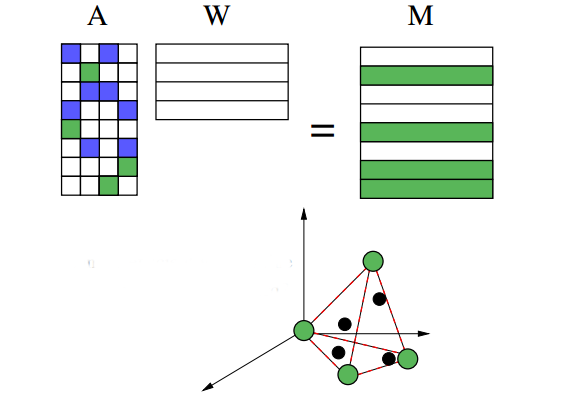
\includegraphics[scale=0.4]{convexhull.png}
\caption{Convex hull formed after joining anchor words \cite{tm}}
\label{fig:convexhull}
\end{figure}
The high level sketch of algorithm as proposed by \cite{tm} is given in \ref{fig:algorithm}.

\begin{figure}[htb]
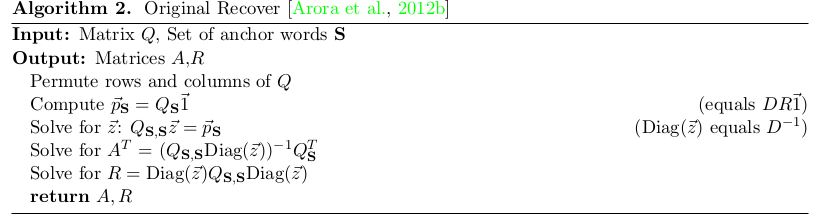
\includegraphics[scale=0.5]{algorithm.png}
\caption{Algorithm for finding Anchor words }
\label{fig:algorithm}
\end{figure}

\section{Dataset}
We have evaluated the results using the subset of Associated Press data set. This data set consists of documents which focus on different content areas and while still being rather small has similar characteristics as other corpora used in the topic models literature. The subset is from the Associated Press data from the First Text Retrieval Conference (TREC-1) and it is available on Blei's web page (http://www.cs.princeton.edu/~blei/lda-c). It consists of 2246 documents and the vocabulary was already selected to contain only words which occur in more than 5 documents. We also considered using New York Times dataset for evaluating our results but it was not freely and readily available.

\section{Methods}
We have mainly focused on the approaches mentioned in paper [1] and tried to implement what they have mentioned. This concept of anchor words, words that helps to decide the topic of a document, is very promising. Though it comes with different inherant problems like it is not easy to find anchor words for every document and sometimes having more documents make it more complex to find anchor words as it might overlap with other documents as well. Despite all this, Anchor words helps to differentiate one document from other contextually. 

Also the authors express doubt over whether matrix factorization version of this algorithm is indeed practical. So instead we followed a probabilistic approach for finding the topic model. Also word-word cooccurence matrix($10,000*10,000$) was too large to contain in memory. Therefore we used the following methods for dimensionality reduction.

\begin{itemize}
\item Principle Component Analysis
\item Random Projection 
\end{itemize} 

We choose random projections over the first method as it was comparatively fast and efficient. It was also easier to customize based on the word-word cooccurence matrix we had. In following subsections the method used for find anchor words and how to use them to recover topics of the documents has been explained. \\

\subsection{Calculating word word co occurrence matrix}
We calculate Word Word covariance matrix as we get very noisy version of data and this matrix has property that  $\hat{M} \hat{M}^T -> M M^T $ and $W W^T -> R$ as number of documents increases. For computation of this matrix we counted number of times each word appears in certain document and formed a document word matrix. We represented this matrix $\bar{Hd}$ as sparse as it had very few number of non zero entries. We normalised all the entries by dividing each count by sqrt(n*n-1) where n is total number of words in that document. We also computed $\hat{H}$ which is diagonal matrix which contains elements total count divided by (n*n-1). Then word word covariance matrix Q is given by equation (1).

\begin{equation}
Q = \bar{H} \bar{H}^T - \hat{H}
\end{equation}
The size of this matrix is very large of order of square of size of dictionary. Even though matrix is sparse it will take a huge amount of space. We solve this problem using random projection of matrices.Random projection is based on Johnson-Lindenstrauss lemma which is explained in section below. We take random projection of word word co occurrence matrix and reduce its size considerably from $O((dictionary size)^2)$ to $O((dictionary size)*P)$. Our dictionary size was around 10473, so we reduced space taken by word word co variance matrix from $O((10473)^2)$ to $O((10473)*500)$.

\subsubsection{Johnson-Lindenstrauss lemma}
Random projection is based on Johnson-Lindenstrauss lemma which is "If points in a vector space are projected onto a randomly selected subspace of suitably high dimension, then the distances between the points are approximately preserved." as stated in \cite{randomProjection} Random projection reduces size of matrix considerably by projecting it to lower dimension, but keeps the distances between two points approximately same as it was in higher dimension.


\subsection{Recovering Word Topic Matrix}
The algorithm we have implemented is based on a probabilistic approach where we find the conditional probabilities of words given topics using Bayes theorem. For this purpose we use the row-normalized word co-occurrence matrix $\bar{Q}$ which gives the conditional probability among pairs of words. So given $\hat{Q_{i}}$, which is a row of the empirical row normalized co-occurrence matrix we wish to find out the $p(z_{1}/w_{1})=i$ which can best recover the rows as a convex combination of the anchor words. This step can be done in parallel using exponentiated gradient algorithm. The word topic matrix can be recovered once we have $p(z_{1}/w_{1})$ using Bayes rule. 


\section{Results}

\subsection{Verifying Separability Assumptions}

From given AP dataset we evaluated our algorithm. Algorithm returned anchor words such as Buenoes, Edt, Chapman, Y, bcspehealth, cdy, cycle, nikkei and heres We take random projection of word word co occurrence matrix and reduce its size considerably from $O((dictionary size)^2)$ to $O((dictionary size)*P)$. Our dictionary size was around 10473, so we reduced space taken by word word co variance matrix from $O((10473)^2)$ to $O((10473)*500)$. This was used to get all anchor words from the algorithm, we checked ourselves to see the topics that these anchors are inclined to. After self-analysis of whole AP dataset, following is our observation based on each anchor word:

Anchor Words {\color{orange} change to table}

\begin{verbatim}
buenos
edt
chapman
y
shevardnadze
bcspehealth
cdy
cycle
nikkei
heres
\end{verbatim}

\begin{enumerate}
\item Buenos: this anchor word talks about Buenos Aires, a city in Argentina where various articles discussed about politics in this city. So topic as per our observation is Politics. 

\item EDT: Topic in this case of Anchor word is Weather as various articles talked about weather updates at various times of the day. 

\item Chapman: This was a confused Anchor word which didn't point to any specific topic as Chapman is used as name of people and places in Articles. 

\item Y: This Anchor word points towards a person "Obando y Bravo" as there are couple of articles in dataset about this person. 

\item Shevardnadze: This anchor word points to a politician Eduard Shevardnadze. Dataset consists of many articles covering Eduard Shevardnadze. Thus, topic for this word is Politics. 

\item Cdy: This points towards weather as this anchor word is specific to few articles talking about weather in various cities. 

\item Cycle: This is very interesting anchor and it points towards agriculture, election and annual cycles mentioned in various articles of a dataset. 

\item Nikkei: It points towards Nikkei stock exchange. 

\end{enumerate}


We also generated topics using Latent Dirchlet Allocation program implemented by David Blei and which is available on his website.  \\


{\color{orange} change to table}
\begin{verbatim}
topic 000
   percent
   million
   year
   billion
   new
   market
   company
   prices
   stock
   last


topic 001
   i
   years
   new
   court
   people
   two
   state
   time
   case
   year


topic 002
   police
   people
   two
   government
   officials
   killed
   military
   three
   miles
   today


topic 003
   bush
   president
   soviet
   government
   states
   united
   i
   new
   party
   house
\end{verbatim}

Comparing the results obtained from LDA, anchor words much more accurately represented the document collection. For instance, letters like 'i' was selected as a topic in multiple documents which doesn't point to any specific topic. We believe that these anchor words will help in recovery of better topics from the documents.


\section{Future Work}

\begin{itemize}

\item Generating Variable-Length topics modelling using sequitur algorithm:
	In existing approaches for topic modelling it only finds topics on length of single word. But this might not necessarily be the case. We would like to find topics of variable length. One approach for doing this is applying topic modelling over rules generated by algorithms like sequitur rather than applying rules over words.

\item Recommendar systems using topic modelling:
	LDA assumes that priors that have the form of the Dirichlet distribution. LDA can applied to predict review scores based on the content of reviews and to uncover implicit community structures in a social network. It can be also extended to include general meta-data of users and objects.

\end{itemize}


\begin{thebibliography}{99}
\bibitem{tm} \textit{Learning Topic Models---Going beyond SVD}. Arora, Saneev, Rong Ge, and Ankur Moitra. In FOCS 2012.
\bibitem{dred} \textit{Online methods for multi-domain learning and adaptation}. Dredze, Mark and Crammer, Koby. In
EMNLP, 2008.
\bibitem{nmf} \textit{Computing a nonnegative matrix factorization--provably}. Sanjeev Arora, Rong Ge, Ravi Kannan, Ankur Moitra. Proceedings of the 44th symposium on Theory of Computing. ACM, 2012.  
\bibitem{blei} \textit{Review article on Probabilistic topic models}. David m. Blei  

\bibitem{pam} \textit{Nonparametric bayes pachinko allocation}. Li, Wei, David Blei, and Andrew McCallum. arXiv preprint arXiv:1206.5270 (2012). 

\bibitem{anand12} \textit{Two svds suffice: Spectral decompositions for probabilistic topic modeling and latent dirichlet allocation}. Anandkumar, Animashree, et al.  arXiv preprint arXiv:1204.6703 (2012).

\bibitem{randomProjection} \textit{Experiments with random projection}. Dasgupta, Sanjoy. Proceedings of the Sixteenth conference on Uncertainty in artificial intelligence.


\end{thebibliography}

\pagebreak


\end{document}